%% bare_jrnl.tex
%% V1.4b
%% 2015/08/26
%% by Michael Shell
%% see http://www.michaelshell.org/
%% for current contact information.
%%
%% This is a skeleton file demonstrating the use of IEEEtran.cls
%% (requires IEEEtran.cls version 1.8b or later) with an IEEE
%% journal paper.
%%
%% Support sites:
%% http://www.michaelshell.org/tex/ieeetran/
%% http://www.ctan.org/pkg/ieeetran
%% and
%% http://www.ieee.org/


\documentclass[journal]{IEEEtran}


\usepackage{times}
\usepackage{epsfig}
\usepackage{graphicx}
\graphicspath{{images/}}
\usepackage[justification=centering]{caption}
\usepackage{subfigure}
\usepackage{float} %插图
\usepackage{amsmath}
\usepackage{amssymb}
\usepackage{multirow}
\usepackage{cite}
\usepackage{bm}%公式文本粗体
\usepackage{hyperref}
\usepackage{xfrac}% 斜分号
\usepackage{booktabs}%表格
\usepackage{array}% 表格
\makeatletter
\newcommand{\rmnum}[1]{\romannumeral #1}
\newcommand{\Rmnum}[1]{\expandafter\@slowromancap\romannumeral #1@}
\makeatother



% correct bad hyphenation here
\hyphenation{op-tical net-works semi-conduc-tor}


\begin{document}

\title{Small Target Detection in Infrared Video \\Based on Spatio-temporal Tensor Model}
%
%
% author names and IEEE memberships
% note positions of commas and nonbreaking spaces ( ~ ) LaTeX will not break
% a structure at a ~ so this keeps an author's name from being broken across
% two lines.
% use \thanks{} to gain access to the first footnote area
% a separate \thanks must be used for each paragraph as LaTeX2e's \thanks
% was not built to handle multiple paragraphs
%

\author{Hongkang~Liu,~Lei~Zhang,~\IEEEmembership{Fellow,~IEEE}
        and~Hua~Huang,~\IEEEmembership{Fellow,~IEEE}% <-this % stops a space
\thanks{M. Shell was with the Department
of Electrical and Computer Engineering, Georgia Institute of Technology, Atlanta,
GA, 30332 USA e-mail: (see http://www.michaelshell.org/contact.html).}% <-this % stops a space
\thanks{J. Doe and J. Doe are with Anonymous University.}% <-this % stops a space
\thanks{Manuscript received April 19, 2005; revised August 26, 2015.}}

% note the % following the last \IEEEmembership and also \thanks - 
% these prevent an unwanted space from occurring between the last author name
% and the end of the author line. i.e., if you had this:
% 
% \author{....lastname \thanks{...} \thanks{...} }
%                     ^------------^------------^----Do not want these spaces!
%
% a space would be appended to the last name and could cause every name on that
% line to be shifted left slightly. This is one of those "LaTeX things". For
% instance, "\textbf{A} \textbf{B}" will typeset as "A B" not "AB". To get
% "AB" then you have to do: "\textbf{A}\textbf{B}"
% \thanks is no different in this regard, so shield the last } of each \thanks
% that ends a line with a % and do not let a space in before the next \thanks.
% Spaces after \IEEEmembership other than the last one are OK (and needed) as
% you are supposed to have spaces between the names. For what it is worth,
% this is a minor point as most people would not even notice if the said evil
% space somehow managed to creep in.



% The paper headers
\markboth{Journal of IEEE Transactions on Geoscience and Remote Sensing,~Vol.~14, No.~8, August~2018}%
{Shell \MakeLowercase{\textit{et al.}}: Bare Demo of IEEEtran.cls for IEEE Journals}
% The only time the second header will appear is for the odd numbered pages
% after the title page when using the twoside option.
% 
% *** Note that you probably will NOT want to include the author's ***
% *** name in the headers of peer review papers.                   ***
% You can use \ifCLASSOPTIONpeerreview for conditional compilation here if
% you desire.




% If you want to put a publisher's ID mark on the page you can do it like
% this:
%\IEEEpubid{0000--0000/00\$00.00~\copyright~2015 IEEE}
% Remember, if you use this you must call \IEEEpubidadjcol in the second
% column for its text to clear the IEEEpubid mark.



% use for special paper notices
%\IEEEspecialpapernotice{(Invited Paper)}




% make the title area
\maketitle

% As a general rule, do not put math, special symbols or citations
% in the abstract or keywords.
\begin{abstract}
Existing methods for infrared small target detection are not effective under highly complex backgrounds condition. It is mainly caused by: (1) the interference of strong edges and other similar-target components. (2) not making full use of the context information of background and target in spatio-temporal domain. Inspired by this, we form a spatio-temporal cube with current image patch and adjacent image patches in spatio-temporal adjacent domain, then we establish a spatio-temporal tensor model for small target detection. According to the sparse prior of target and the local correlation of background, the target-background separation problem is transformed into a low rank-sparse tensor decomposition problem. The target image is reconstructed from the sparse tensor obtained after tensor decomposition. The experiment results show that our method could make full use of the context information in spatio-temporal domain in infrared video. Compared with other methods, our method has better detection performance in several videos with highly complex backgrounds.
\end{abstract}

% Note that keywords are not normally used for peerreview papers.
\begin{IEEEkeywords}
Infrared video, small target detection, spatio-temporal tensor model, tensor decomposition.
\end{IEEEkeywords}


%Intruction
%
%

\section{Introduction}

\IEEEPARstart{A}{t} present, infrared target detection technology has been widely used in missile tracking, precision guidance, early warning, maritime surveillance, ground monitoring\cite{luo2015space,dawson2010space,li2014infrared}, etc. Compared with ordinary detection tasks, lacking of sufficient information to determine the target is the main challenge of small target detection in infrared image. Due to the long infrared imaging distance, the size of small targets in infrared image is very small, generally ranging from $2\times2$ to $9\times9$ pixels\cite{wang2017infrared}. And in the case of long imaging distance, the small targets in infrared image has no fixed shape and stable texture features. In addition, the infrared radiation of targets is heavily attenuated after long-distance propagation, which results in a low signal-to-noise ratio (SNR) for small infrared targets\cite{li2016novel}. When there are complex background clutter and noise, small targets with low signal-to-clutter ratio (SCR) are usually buried in background. Therefore, the detection of small targets under a complex infrared background is remaining a problem that is full of difficulty and challenges.

Compared with visible image, infrared image look simpler. However, infrared image lacks color information and texture information, and has poor image quality usually, which cause great difficulty in the process of small target detection.The lack of color information will result in fewer features for distinguishing between target and background. The lack of texture information and shape information means that the target cannot be distinguished based on the feature learning of the small target. Therefore, utilizing not only the relationship between small target and background, but also the motion characteristics of target is an important way to detect infrared small targets.

The small target detection methods in infrared image are mainly divided into two categories: single-frame image detection methods which use spatial domain information and spatio-temporal detection methods which utilize inter-frame temporal domain information and intra-frame spatial domain information\cite{li2016novel}. There are often some special backgrounds, such as man-made objects and cloud patch, which will interfere with the target detection task, and the imaging resolution and SCR of small target are smaller than expected. Therefore, it is impossible to identify target by using only the information in spatial domain, and the small target on a single image is invisible in perception. According to above analysis, it is extremely important to make full use of the context information of small target in the temporal domain. The current spatio-temporal detection methods usually calculate the local contrast of spatial domain and temporal domain separately, and combines them to detect the small target. However only calculating of local contrast will not identify true small targets in the case of complex noise or the motion of background, resulting in excessive false alarms and missing alarms. In order to make full use of the effective information of temporal domain and spatial domain, and to avoid the influence of noise when detecting, we propose a method for small target detection based on spatio-temporal image patch tensor decomposition. The main contribution of this paper is as follows: The proposed spatio-temporal tensor model considers the local correlation of the background image patch in spatial and temporal neighborhood domain, so it will suppress the background clutter better. And our method not only reflects the spatial significance of target, but also make full use of the motion characteristics of small target, utilizing the sparse characteristics of small target in spatio-temporal neighborhood domain.

The remaining chapters of this paper are organized as follows: We introduce the related researches of infrared small target detection in section \Rmnum{2}; And in section \Rmnum{3} we propose the spatio-temporal tensor model and the method for detecting infrared small targets via spatio-temporal image patch tensor model in detail; In section \Rmnum{4},we verify the effectiveness of the proposed method via a large number of experiments; In section \Rmnum{5}, we give the conclusions and prospects for future.

%Related work
%
%
\section{Related Work}
At present, the methods proposed for detecting small moving targets in infrared video can roughly classified into two categories. The first major category is mainly performing target detection on a single image. Another category detect small targets utilizing multiple images from a infrared video.

\subsection{Detection Methods Based on Single Image}
The methods for target detection via single image frame are further divided into two types, which are based on the following two assumptions. The first type of methods are based on a classic assumption that background changes slowly in infrared images and high correlations exist between adjacent pixels. Another type of methods based on single image frame utilize the non-local self-correlation between background pathes in infrared image. It is usually assumed that all background image patches in infrared image are from a low-rank subspace or a mixed set composed with multiple low-rank subspaces\cite{liu2013robust}.

Based on the first hypothesis, some classical methods based on image filtering are proposed, such as two-dimensional minimum mean square error filtering\cite{hadhoud1988two}, maximum median and maximum mean filtering\cite{deshpande1999max}, transform domain methods \cite{davidson2002wavelet,peng2004dim} and so on. This type of methods enhance small targets by calculating the difference between original image and predicted background. Other methods have been proposed with extensive research in human visual system, such as Laplacian Gaussian (LoG) filter based methods\cite{kim2009small}, Gaussian difference (DoG)\cite{wang2012infrared} and second-order directional derivatives\cite{qi2013robust}. Although this type of methods can reduce the influence of edge compared with traditional method, it can not suppress the clutter and strong edges in complex background, resulting in many false alarms. Meanwhile, there is usually a large difference between infrared small target and surrounding background, based on which some methods based on local contrast are proposed, such as local contrast measurement method (LCM)\cite{chen2014local}, improved local contrast measurement (ILCM)\cite{han2014robust}, image block based multi-scale contrast measurement (MPCM)\cite{wei2016multiscale} and so on. Similarly, other methods such as local difference measurement (LDM)\cite{deng2017entropy}, local significance map (LSM)\cite{chen2016efficient} and weighted local difference measure (WLDM)\cite{deng2016small} have been proposed in succession. This traditional type of methods can suppress background and enhance small targets, but a large amount of noise and clutters are also enhanced in the case of complex background, and are considered as small targets by mistake. So the false-alarm rate of these methods are usually high and the practicability is reduced also.

Based on the second hypothesis, small target detection in infrared image can be transformed into a low-rank matrix recovery problem. Gao\cite{gao2013infrared} et al. proposed to convert the traditional infrared image model into a new infrared image patch model, and considered that background has low rank characteristics and the small targets are sparse relative to the whole image. Therefore target could be separeated from background via recovering low-rank and sparse matrices. However, the method still has insufficient effect when processing strong edges and clutters, so RIPT\cite{dai2017reweighted} extract prior features via local structure information , and then suppress edges with local structure weight in the process of small target detection. However in the case of complex background, the image patches may come from multiple low-rank subspaces, so Wang\cite{wang2017infrared} et al. use a multiple-subspace learning strategy to better suppress background, whih can effectively reduce false alarm rate. The above methods are based on robust principle component analysis (RPCA) to achieve small target detection. But, due to the existence of many clutters in background in single image, such as cloud patches in sky and fixed heat objects on ground, the detection of true targets will be interfered seriously. The information of single image is not sufficient to identify small targets, so it is necessary to take temporal information into account including motion information of target and context information of background.

\subsection{Detection Methods Based on Multiple Images}
The second major mathods for infrared small targets detection are mainly based on multiple images from infrared video. These methods make full use of information in spatial domain ton suppress background clutters and utilize motion characteristics of targets to highlight small targets. Therefore better detection results could got. Silverman and Caefer et al. utilized temporal information for small target detection, and proposed Recursive Variance Filter (TVF)\cite{silverman1998temporal} and Damped Sinusoid Filters (TTF)\cite{caefer1998temporal}. But the difference of target and moving background can not be reflected according to temporal information only. For example, moving cloud may be detected as true target. And then Deng et al.\cite{deng2016infrared} proposed a spatial-temporal local contrast filter for infrared small target detection, but the calculation of local contrast via pixels is easily affected by noise. Gao et al. proposed TVPCF\cite{gao2017tvpcf} which combines multi-scale local contrast based on patches with temporal filter to obtain better detection results. Li et al.\cite{li2016novel} proposed a new way to calculate local contrast. Image patches in spatio-temporal neighborhood of current image patch are used to reconstruct a new image patch. The residual of current image patch and reconstructed image patch is defined as local contrast. Although this method can suppress clutters and single pixel noise, the reconstruction process is extremely sensitive ton noise. Therefore many targets will be missed under high noise.

\begin{figure*}[htb]
  \centering
  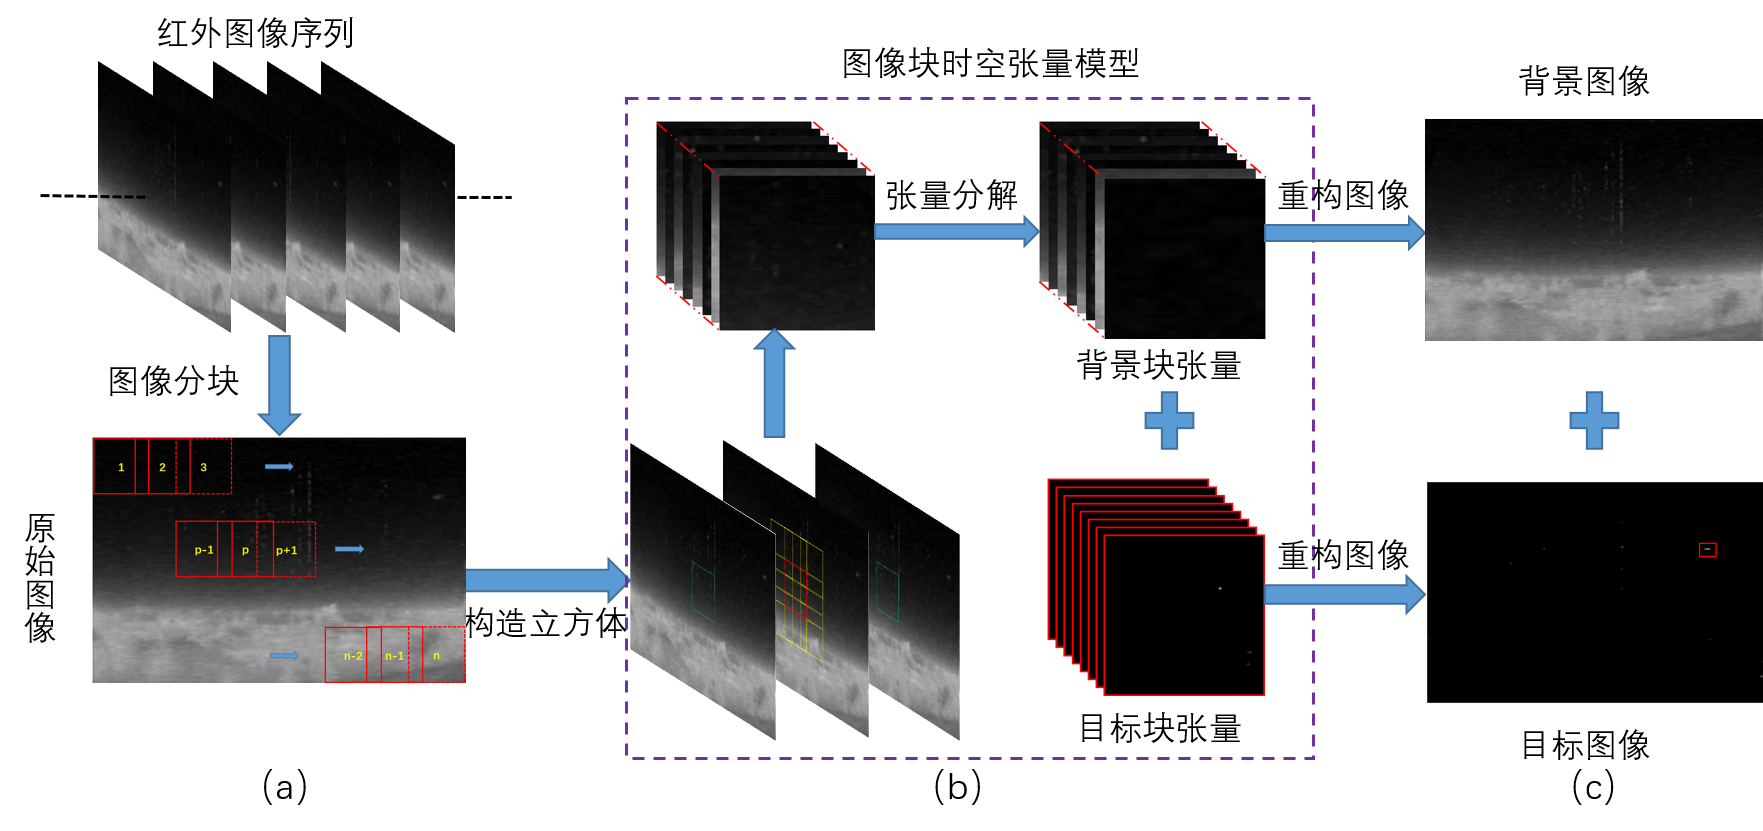
\includegraphics[width=0.9\textwidth]{flow_chart.png}
  \caption{The flow chart of small target detection based on spatio-temporal tensor model}
  \label{fig:flow_chart}
\end{figure*}


\section{Construction and Decomposition of Spatio-temporal Tensor Model}
Due to the traditional imaging mechanism, there is usually a strong correlation between background image patches in spatial adjacent domain. And background moves slowly compared with target, so background image patches also have strong correlations in temporal adjacent domain. Then, single image is segmented into image patches by sliding window, and an image patch cube is formed by current patch and patches from the spatial and temporal adjacent domain of current patch. The image patch cube is viewed as a spatio-temporal tensor. In the spatio-temporal tensor, background tensor is low-rank and target tensor is sparse. Therefore the target tensor can be decomposed from original tensor, then target patch is separated from original patch. The specific construction method and decomposition process of spatio-temporal tensor model will be described in detail in this section.


\subsection{Construction of spatio-temporal tensor model}
In order to make more use of the relevant information between backgrounds in infrared frames, we propose a new target and background separation model called the spatio-temporal tensor model in this section. Usually, the infrared image model is defined as follows for infrared small target detection similar to\cite{gu2010kernel}:
\begin{equation}
  f_D(x,y)=f_T(x,y)+f_B(x,y)+f_N(x,y)
  \label{eq:image_model}
\end{equation}
where $f_D,f_T,f_B,f_N \text{ and } (x,y)$ corresponds to the original infrared image, the target image, the background image, the noise image and the position coordinates of each pixel respectively.

Figure 1(a) shows the construction process of spatio-temporal image patch tensor. Firstly, the original image is divided into several image patches via sliding window from top to bottom and left to right. For each image patch, $m_t$ image patches in temporal adjacent domain and $m_s$ image patches in spatial adjacent domian (including itself) are collected to form a spatio-temporal cube. The spatio-temporal cube is also viewed as a tensor called spatio-temporal image patch tensor. Spatial image patch tensor and temporal image patch tensor are constructed 
as shown in figure 1(b):
\begin{equation}
  \begin{split}
    \bm{D}_t = \bm{B}_t + \bm{T}_t + \bm{N}_t \\
    \bm{D}_s = \bm{B}_s + \bm{T}_s + \bm{N}_s
  \end{split}
\end{equation}
where $\bm{D}_t,\bm{B}_t,\bm{T}_t,\bm{N}_t \in R^{{I}\times{J}\times{m_t}}$ are the tensors composed with original image patches, background image patches, target image patches and noise image patches from spatial adjacent domain separately. Moreover, $\bm{D}_s,\bm{B}_s,\bm{T}_s,\bm{N}_s \in R^{{I}\times{J}\times{m_s}}$ are are the tensors composed with original image patches, background image patches, target image patches and noise image patches from temporal adjacent domain separately. $I\text{ and }J$ correspond to the height and width of image patch, respectively, depending on the size of sliding window. Then, the context information in spatial and temporal adjacent domain could be utilized by us at the same time, so the following tensor model can be formed by combining the spatial and temporal tensor mentioned above:
\begin{equation}
  \bm{D}=\bm{B}+\bm{T}+\bm{N}
\end{equation}
where $\bm{D},\bm{B},\bm{T},\bm{N} \in R^{{I}\times{J}\times{(m_t+m_s)}}$.

The context information of background in temporal domain and spatial domain can be utilized simultaneously according to the above model. Nextly, we will analyze the characteristics of each component in spatio-temporal image patch tensor in detail. And we will give the solution algorithm for our spatio-temporal tensor model on the basis of classical low-rank tensor recovery algorithm to detect small targets in infrared video.

\subsection{Background image patch tensor $\mathbf{B}$ }
In general, the movement of background is slow relative to small targets, so there are high correlations between background image patches in temporal neighborhood. Moreover, the imageing principium in infrared video causes that the image patches are also correlated within spatial local neighborhood. At present, the most advanced IPI\cite{gao2013infrared} model adopts the non-local correlation of background image patches, but we adopt the local correlation of them. The reason why we adopt the local correlation of background image patches is that the local correlation is stronger than non-local.

In order to compare with traditional IPI model for convenience, our spatio-temporal tensor model selects several background image patches in spatio-temporal adjacent domain, and the IPI model randomly selects same number of background image patches of non-local regions. Then we transform the spatio-temporal tensor into a mode-1 unfold matrix. And the singular values are calculated of the matrixs formed by two models. It can be seen from the first and second rows of figure(2) that the singular valuse of spatio-temporal tensor which utilizes the local correlation of background image patches decrease faster. It proves that the background tensor in our model has better low-rank characteristics, so it can be ensured that there will be fewer background components (clutters) in targetb tensor during the decomposition process.
\begin{figure}[H]
  \centering
  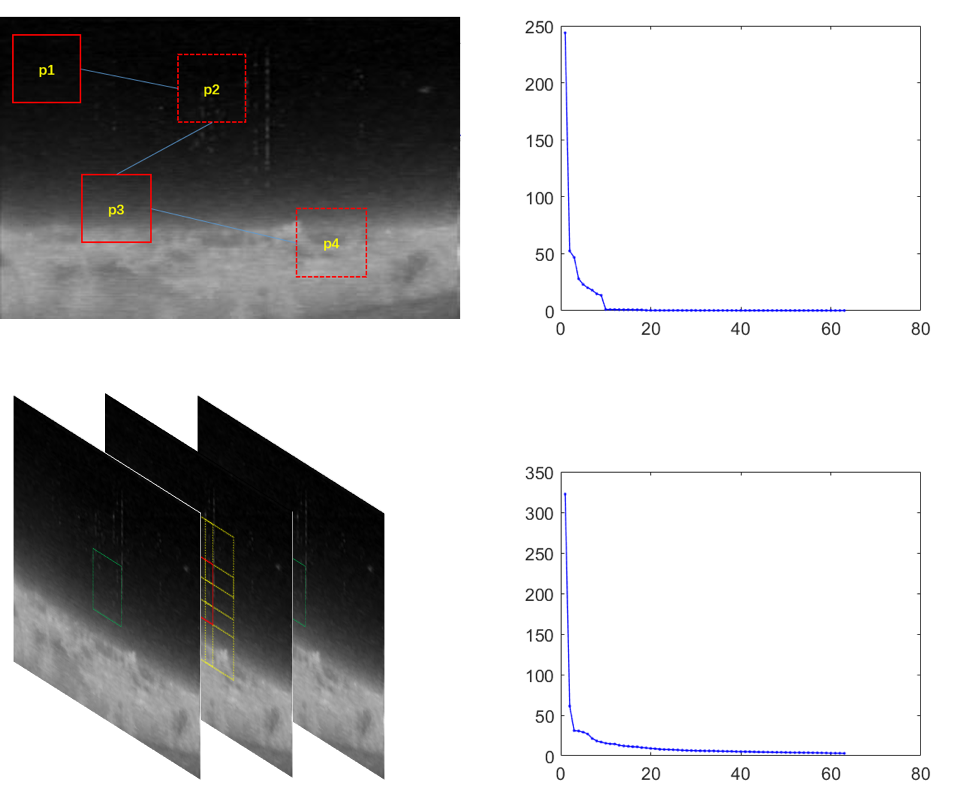
\includegraphics[width=0.5\textwidth]{singular.png}
  \caption{First row: singular value curve of non-local correlation;Second row:singular value curve of local correlation}
  \label{singular}
\end{figure}

From the above analysis, we know that the background tensor is low-rank:
\begin{equation}
  rank(\bm{B}) \leq r
\end{equation}
where $r$ is a low-rank constant constraint corresponding to background tensor. Usually $r$ is bigger in complex background than uniform background.


\subsection{Target Image Patch Tensor $\mathbf{T}$}
In actual application scenario, due to the infrared imaging characteristics, there is no obvious texture information and color information of small targets in infrared video. And the sizes of different targets also vary within a certain range. Moreover, the brightness of infrared small target is also different in different scenes. But infrared small targets are always small in size because of that imaging distance is far. So if small target appears in spatio-temporal patch cube, the volume occupied by small target is great smaller compared with the volume of entire spatio-temporal patch cube. Specifically expressed as follows:
\begin{equation}
  V(\bm{T}) \ll V(\bm{D})
\end{equation}
Therefore, the target image patch tensor is a sparse tensor actually, and it satisfies:
\begin{equation}
  \left \| \bm{T} \right \|_0 \leq k
\end{equation}
where $k$ is a small constant that can be visually regarded as the volume corresponding to target, which is determined by the size of the target and the number of times that targets appear in the spatio-temporal patch cube.

\subsection{Noise Image Patch Tensor $\mathbf{N}$}
As mentioned in\cite{gao2013infrared}, random noise in infrared video is generally considered to be independent and identically distributed Gaussian white noise. And for a given $\delta>0$, noise image patch tensor satisfies $\left \| \bm{N} \right \|_F \leq \delta$. So according to formula (3), we can get the following restriction:
\begin{equation}
  \left \| \bm{D}-\bm{B}-\bm{F} \right \|_F \leq \delta.
\end{equation}
The $r,k,\delta$ vary in different image tensor, but we will not utilize the specific values of them.


\subsection{The Decomposition Method for Spatio-temporal Image Patch Tensor}
The ultimate goal of us is to detect small targets in infrared video, so we need to get the target image $f_T$ based on the original image $f_D$ given. As shown in figure 1(c), the current target patches of all target tensors corresponding to entire original image can be reconstructed to obtain the target image, so it is critical to attain the target tensor from original spatio-temporal tensor.

We first assume that there is no noise in original infrared image, then the original image consists of background image and target image, expressed in the tensor model as $\bm{D}=\bm{B}+\bm{T}$. According to the above discussion, we know that the background image patch tensor is low-rank and the target image patch tensor is sparse. So we can attain target image patch tensor and background image patch tensor from tensor decomposition. And then, we can reconstruct the target image from all target image patch tensors. Therefore, the original target detection problem is transformed into the following optimization problem according to our model:
\begin{equation}
  \underset{\bm{B},\bm{T}}{min} \ rank(\bm{B}) + \lambda \left \| \bm{T} \right \|_0 \ s.t. \bm{D}=\bm{B}+\bm{T}
  \label{min_1}
\end{equation}
But the optimization problem is a NP-hard problem, and it is impossible to calculate the rank of background image patch tensor. Therefore, this paper adopts nuclear norm $\left \| \bm{B} \right \|_*$ to restrict background image patch tensor instead of low-rank constraint. At the same time, in order to facilitate the calculation, we substitute $l_0$ norm with $l_1$ norm of target tensor. Then, we consider that noise tensor satisfies $\left \| \bm{N}\right \|_F \leq \delta$. So, the optimization problem in equation (\ref{min_1}) can be transformed into following convex optimization problem:
\begin{equation}
  \underset{\bm{B},\bm{T}}{min} \ \left \| \bm{B} \right \|_* + \lambda \left \| \bm{T} \right \|_1 \ s.t. \left \|\bm{D}-\bm{B}-\bm{T} \right \|_F\leq \delta
  \label{min_2}
\end{equation}
The $\lambda$ parameter mentioned above plays a balancing role between background tensor and target tensor. A large $\lambda$ not noly reduce the non-target components in target tensor, but also cause that the target components in target tensor shrink excessively because of which some targets will be missed. Conversely, a small $\lambda$ will increase the target component in target tensor, but the non-target component in target tensor may also increase so much resulting in some clutters alarmed by mistake. Therefore, it is important to choose a appropriate $\lambda$ for target detection. In this paper, the $\lambda$ is determined according to both the size of image patch and the number of selected image patches for spatio-temporal tensor construction. The detail for selection of $\lambda$ will be described in experiment section.

Solving the tensor decomposition problem utilizing ADMM algorithm mentinoed in \cite{dai2017reweighted}, the augmented lagrangian expression of the formula (\ref{min_2}) is as follows:
\begin{equation}
  \begin{split}
    L & = \left \|\bm{B} \right \| _* +\left \|\bm{B} \right \| _1 + \\
    & \frac{1}{2\mu} \left \|\bm{D}-\bm{B}-\bm{T} \right \| ^2 - \langle\bm{Y},\bm{B}+\bm{T}-\bm{D}\rangle
  \end{split}
\end{equation}
Then, according to the solution method proposed in\cite{dai2017reweighted}, the background tensor and the target tensor can be obtained by minimizing the augmented lagrangian function.


\subsection{The Detection Process Based on Spatio-temporal Tensor Model}
As shown in figure (\ref{fig:flow_chart}), the main process of detection method proposed in this paper is 
divided into four steps:
\begin{itemize}
  \item [(1)]According to the prescribed step size, the original image is divided into several image blocks by sliding window from top to bottom and left to right.
  \item [(2)]During the window sliding process, a current original spatio-temporal cube is obtained formed with current image patch and patches in its spatial and temporal adjacent domain. And the cube is viewed as a spatio-temporal image patch tensor.
  \item [(3)]According to the solution method mentioned above, the corresponding background image patch tensor and target image patch tensor are decomposed from the original spatio-temporal image patch tensor. So we can obtain the target and background image patch corresponding to current original image patch.
  \item [(4)]The target image and background image can be reconstructed from target patches and background patches with a sliding window passes through the entire orignal image.
\end{itemize}
According to the above detection process, good results can be obtained. And small targets in complex background can be accurately detected. In addition, we think that some post-processing methods could improve detection result significantly. But we adopt none post-processing method in our experiment part to compare the advantages and disadvantages of each detection method for infrared small targets.


\section{Experiment And Analysis}
In order to reflect the effectiveness and advancement of our mathod, we compare our mathod with five detection methods of different types in experimental part. The proposed method utilizes both spatial and temporal information, so it is firsty compared with three detection methods that only use spatial domain information, namely MPCM method\cite{wei2016multiscale}, IPI method\cite{gao2013infrared} and RIPT method\cite{dai2017reweighted}. And then, we also compare our method with two detection methods which utilize both spatial and temporal information in infrared video, namely STLCF method\cite{deng2016infrared} and the method proposed by Li et al\cite{li2016novel}. We analyze the performance of each detection method on different data sets.

\subsection{Measurement Metrics}
The measurement metrics used in our experiments reference the metrics defined in\cite{gao2013infrared}\cite{dai2017reweighted}. But we adjust the scope of adjacent domain of target as $d=40$. The measurement metrics are defined as follows.

SCR is one of the most common measurement metrics, usually used to measure the difficulty of small target detection. The calculation formula is defined as follows:
\begin{equation}
  SCR=\frac{\left| \mu_t -\mu_b \right|}{\sigma_b}
  \label{SCR}
\end{equation}
where $\mu_t \text{ and }\mu_b$ are the mean pixel intensity of target domain and background adjacent domain respectively. And $\sigma$ is the standard deviation of background area. According to \ref{SCR}, SCR gain is defined as:
\begin{equation}
  SCR_{gain}=\frac{SCR_{out}}{SCR_{in}}
\end{equation}
where $SCR_in$,$SCR_out$ are the $SCR$ value of original infrared image and the output image after detection process.

The second measurement metric is background suppression rate, which is defined as follows:
\begin{equation}
  BSF=\frac{\sigma_{in}}{\sigma_{out}}
\end{equation}
where $\sigma _{in}$ and $\sigma _{out}$ are the standard deviation of input image and output image. Another metric is the gain of local signal to noise ratio($LSNR_{gain}$). Firstly, $LSNR$ is defined as $LSNR=\sfrac{I_t}{I_b}$, where $I_t$ and $I_b$ represents the maximum intensity of target area and background area, respectively. So $LSNR_{gain}$ is defined as:
\begin{equation}
  LSNR_{gain}=\frac{LSNR_{out}}{LSNR_{in}}
\end{equation}

In addition to the above metrics, we also calculated the probablity of detection rate and false alarm rate, which are defined as follows:
\begin{equation}
  P_d=\frac{number\;of\;true\;detections}{number\;of\;actual\;targets}
\end{equation}
\begin{equation}
  F_a=\frac{number\;of\;pixels\;of\;false\;detections}{number\;of\;pixels\;in\;all\;images}
\end{equation}
The ROC curve is drawn based on the above two metrics, where $F_a$ is abscissa axis and $P_d$ is ordinate axis.


\subsection{Infrared Video Sets}
In order to verify the effectiveness of our method for small target detection and compare it with other detection methods, the proposed method and other classical detection methods are tested on both the simulated dataset and the real dataset. The results were compared with each other and we summarize the advantages and disadvantages of various detection methods. The infrared videos and infrared background videos utilized in this paper were all taken with the iRay series LA6110 uncooled infrared camera by us. Next, we will introduce the two video sets separately.

\begin{table*}[ht]
  \centering
  \caption{scene introduction of simulation video set}
  \label{tab1}
  \begin{tabular}{|c|m{3cm}<{\centering}|m{3cm}<{\centering}|m{3cm}<{\centering}|m{3.2cm}<{\centering}|}
    \hline
    &Seq1 &Seq2 &Seq3 &Seq4\\
    \hline
    representative video frame& 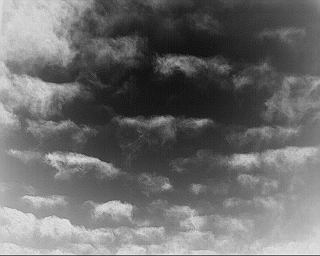
\includegraphics[scale=0.33]{back1.png}& 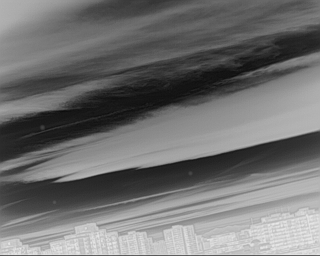
\includegraphics[scale=0.25]{back2.png}& 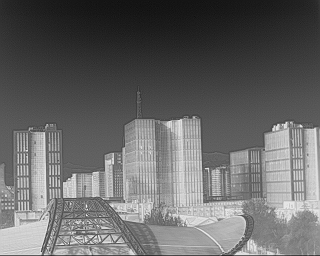
\includegraphics[scale=0.33]{back3.png}& 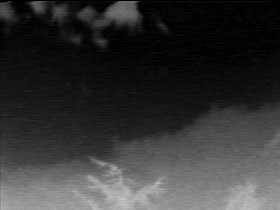
\includegraphics[scale=0.3]{back4.png}\\
    \hline
    size($width \times height$)& $320 \times 256$& $320 \times 256$& $320 \times 256$& $280\times 210$\\
    \hline
    Scene description& Sky scene with complex clouds moving constantly & Sky scene full filled with clouds and some buildings & Complex buildings scene with much interference & Clouds and tree branches are moving quickly due to gale\\
    \hline
    noise level & small & medium & big & big \\
    \hline
    target number & 1 & 3 & 2 & 2 \\
    \hline
  \end{tabular}
\end{table*}


\begin{table*}[ht]
  \centering
  \caption{scene introduction of real video set}
  \label{tab2}
  \begin{tabular}{|c|m{3cm}<{\centering}|m{3cm}<{\centering}|m{3cm}<{\centering}|m{3.2cm}<{\centering}|}
    \hline
    &Seq1 &Seq2 &Seq3 &Seq4\\
    \hline
    representative video frame& 
    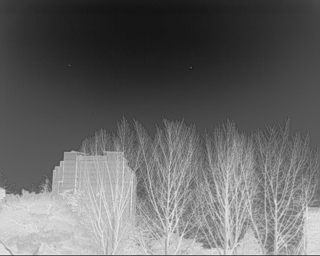
\includegraphics[scale=0.26]{real-back1.png}& 
    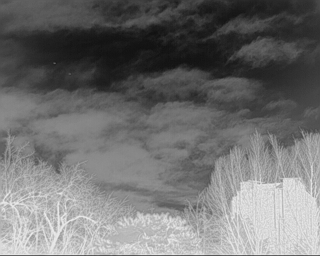
\includegraphics[scale=0.26]{real-back2.png}& 
    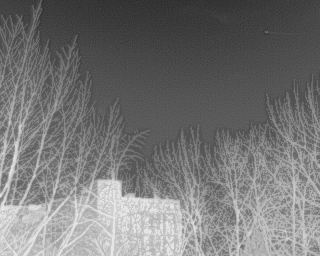
\includegraphics[scale=0.26]{real-back3.png}& 
    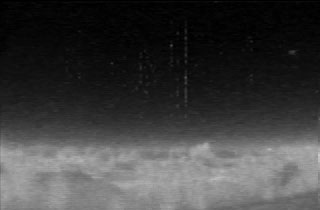
\includegraphics[scale=0.29]{real-back4.png}\\
    \hline
    size($width \times height$)& $320 \times 256$& $320 \times 256$& $320 \times 256$& $320\times 210$\\
    \hline
    Scene description& Sky scene with buildings and trees, no cloud & Sky scene full filled with clouds and trees & Include buildings and tree branches & A single plane gradually disappears behind the horizon\\
    \hline
    noise level & small & medium & big & big \\
    \hline
    target number & 2 & 2 & 1 & 1 \\
    \hline
    target & birds & birds & plane & plane \\
    \hline
  \end{tabular}
\end{table*}

Simulation video set: First, we used infrared camera to shoot four different scenes as background. The information of four scenes are described in table 1. The four scenes selected in this paper represent various scenarios common to infrared small target detection. They can well represent the complex background existing in infrared small target detection. Then, the targets corresponding to each scene described in table \ref{tab1} are added to each video with Poisson fusion strategy\cite{perez2003poisson} according to different motion trajectories.

Real video set: The real video set is divided into two types: sky background and sky background with other interference. The detailed scene information of real video set is given in Table \ref{tab2}.

To fully validate the validity of our detection method, all infrared videos utilized in experiments have highly complex background. It can be seen from the video frames shown in Table 1 and Table 2 that there are a large number of target-like interference components in infrared videos indeed, such as plaque clouds, tree branches, buildings and some high noise.

%插图,实验结果
\begin{figure*}[ht]
  \centering
  \includegraphics[scale=0.55]{result1.eps}
  \caption{The results of six methods on simulation video set. The first column is original frames. The results int first line are corresponding to IPI, MPCM, RIPT from left to right. The results in second line are corresponding to STLCF, STSA, ours from left to right}
  \label{result1}
\end{figure*}

\begin{figure*}[ht]
  \centering
  \includegraphics[scale=0.55]{result2.eps}
  \caption{The results of six methods on real video set. The first column is original frames. The results int first line are corresponding to IPI, MPCM, RIPT from left to right. The results in second line are corresponding to STLCF, STSA, ours from left to right}
  \label{result1}
\end{figure*}

\subsection{Comparsion of Detection Method on Infrared Video Set}
\subsubsection{Detection Results}
We performed six detection methods on different scenes of our video set. In order to show the detection results of different methods directly, we only show the detection results of the representative video frames mentioned in table \ref{tab1} and \ref{tab2}. The detection results of six methods on simulation video set are shown in figure result1. And, the detection results of six methods on real video set are shown in figure result2.

It can be seen from Fig. result1 that the methods such as IPI, MPCM and RIPT have poor results on cloud plaques, building interference and other target-like objects. And many plaque clutters exist common in the target images obtained. Due to utilize the information in spatial domian, the target-like objects appearing in single image tend to be detected as true targets. So, the false alarm of these methods are higher then other methods. Then, the traditional methods based on local spatio-temporal contrast, STLCF and STSA, have bad results when processing moving background. There are many targets missed in the results obtained by STSA, as shown in figureresult1(a,d). STLCF method is sensitive to pixel noise, so there is a lot of noise in the detection results, as shown in figure result2(c,d). Our method obtains good results on simulation video set seen from figureresult1.

It can be seen from figureresult2 that the methods including IPI and MPCM also view the cloud plaques and the bright spots of buildings as true targets mistakenly. Though RIPT can suppress strong edges effectively, it is difficult to recognize
 target-like spots. Due to the noise of video is small and the movement of background is not obvious, STLCF and STSA have better results than single image based detectin methods, as shown in figureresult2(a,b). But there are still small number of missed targets and false alarms in detection results. Howerer, it can be seen from figureresult2, the method proposed by us has good results in four real videos.

 

 \subsubsection{Measurement Metrics}
We also measure the results obtained from six detection methods via the metrics mentinoed above. The measurement metrics of simulation video set are shown in table3. Meanwhile, the measurement metrics of real video set are shown in table4.

It can be seen from Tables 3 and 4 that our detection method has higher $SCR_g$, $LSNR_g$ and $BSF$. It proves that the method proposed by us can highlight targets and suppress backgrounds better in infrared small target detection process. Some metrics corresponding to low-rank sparse tensor separation based methods including IPI, RIPT and our method are too large,even approaching infinity. It is common because of that the noise of adjacent domain is removed so that the standard deviation of noise in adjacent background reduced to zero. In general, our method gets better measurement metrics than other methods.



\subsubsection{ROC Curve}
The ROC curves of six methods on infrared video set are given in figure (ROC). It can be seen from Figure (ROC) that the curves corresponding to our method always rise at the fastest speed, which means that compared with other algorithms, our method can achieve the same accuracy as other methods with a smaller false alarm rate. Moreover, when the accuracy rate reaches maximum value, the false positive rate corresponding to our method is the smallest among all methods. It proves that the the method proposed by us can effectively eliminate noise and avoid the influence of target-like clutters. The ROC curves obtained by STSA method are usually at the bottom and raise slowly. The main reason for this phenomenon is that the method is greatly affected by noise and background motion. In the case of obvious noise, the method of image patch reconstruction is not feasible. And then, the curves of STLCF method raise significantly slower in scenes with large noise. Therefore, the false alarm rate of STLCF is much higher than other methods. It can also be seen from figure (ROC) that our method perform better than single image based methods including IPI, MPCM and RIPT due to the existence of cloud plaques, building sopts and other target-like objects.


\section{Conclusion}
We propose an infrared small target detection method based on spatio-temporal tensor model. The method can not only utilize the information in spatial domain to highlight the target, but also can fully utilize the context information in temporal domain to detect the target accurately. And our method performs good in different scenes.

Based on the method proposed in this paper, we need to slide a window continuously and construct spatio-temporal image patch cubes with image patches in spatio-temporal adjacent domain. During the whole detection process, it is necessary to construct image patch tensors continuously and obtain the sparse tensors. So our method runs slightly slower. Therefore, the next work is to optimize the method proposed in this paper and increase the detection speed.





% if have a single appendix:
%\appendix[Proof of the Zonklar Equations]
% or
%\appendix  % for no appendix heading
% do not use \section anymore after \appendix, only \section*
% is possibly needed

% use appendices with more than one appendix
% then use \section to start each appendix
% you must declare a \section before using any
% \subsection or using \label (\appendices by itself
% starts a section numbered zero.)
%


\appendices
\section{Proof of the First Zonklar Equation}
Appendix one text goes here.

% use section* for acknowledgment
\section*{Acknowledgment}
The authors would like to thank...


% Can use something like this to put references on a page
% by themselves when using endfloat and the captionsoff option.
\ifCLASSOPTIONcaptionsoff
  \newpage
\fi



% trigger a \newpage just before the given reference
% number - used to balance the columns on the last page
% adjust value as needed - may need to be readjusted if
% the document is modified later
%\IEEEtriggeratref{8}
% The "triggered" command can be changed if desired:
%\IEEEtriggercmd{\enlargethispage{-5in}}

% references section

% can use a bibliography generated by BibTeX as a .bbl file
% BibTeX documentation can be easily obtained at:
% http://mirror.ctan.org/biblio/bibtex/contrib/doc/
% The IEEEtran BibTeX style support page is at:
% http://www.michaelshell.org/tex/ieeetran/bibtex/
%\bibliographystyle{IEEEtran}
% argument is your BibTeX string definitions and bibliography database(s)
%\bibliography{IEEEabrv,../bib/paper}
%
% <OR> manually copy in the resultant .bbl file
% set second argument of \begin to the number of references
% (used to reserve space for the reference number labels box)
\bibliographystyle{IEEEtran}
\bibliography{ref}
% biography section
% 
% If you have an EPS/PDF photo (graphicx package needed) extra braces are
% needed around the contents of the optional argument to biography to prevent
% the LaTeX parser from getting confused when it sees the complicated
% \includegraphics command within an optional argument. (You could create
% your own custom macro containing the \includegraphics command to make things
% simpler here.)
%\begin{IEEEbiography}[{\includegraphics[width=1in,height=1.25in,clip,keepaspectratio]{mshell}}]{Michael Shell}
% or if you just want to reserve a space for a photo:

\begin{IEEEbiography}{Hongkang Liu}
Biography text here.
\end{IEEEbiography}

% if you will not have a photo at all:
\begin{IEEEbiographynophoto}{Lei Zhang}
Biography text here.
\end{IEEEbiographynophoto}

% insert where needed to balance the two columns on the last page with
% biographies
%\newpage

\begin{IEEEbiographynophoto}{Hua Huang}
Biography text here.
\end{IEEEbiographynophoto}

% You can push biographies down or up by placing
% a \vfill before or after them. The appropriate
% use of \vfill depends on what kind of text is
% on the last page and whether or not the columns
% are being equalized.

%\vfill

% Can be used to pull up biographies so that the bottom of the last one
% is flush with the other column.
%\enlargethispage{-5in}



% that's all folks
\end{document}


